\documentclass{article}
\usepackage{setspace}
\usepackage{graphicx}
\usepackage{subfigure}
\usepackage{amsmath}
\usepackage{pythonhighlight}
\usepackage{longtable}
\usepackage{booktabs}
\usepackage{geometry}
\usepackage{xcolor}
\usepackage{caption}
\usepackage{amsfonts,amssymb}
\usepackage{multirow}
\usepackage{subfigure}
\geometry{a4paper,scale=0.8}
\begin{document}
\begin{titlepage}
	\begin{center}
		\vspace*{1cm}
		\Large{\textbf{DSA5103}}\\
		\Large{\textbf{Optimization algorithms for data modelling}}\\
		\vspace{1cm}
		\small
		National University of Singapore\\
		Data Science and Machine Learning Department\\
		\today \\
		\vfill
		%School of Mathematics and Science\\
		%Soochow University \\
		%\line(1,0){400}\\[1mm]
		\LARGE{\textbf{Assignment 3}}\\[5mm]
		%\Large{\textbf{-The Research on Students' Admission-}}\\[1mm]
		%\line(1,0){400}
		\vfill
		\small
		Wang Jiangyi, A0236307J\\
		e0732857@u.nus.edu
	\end{center}
\end{titlepage}
\section{Intersection of two convex sets via ADMM}
Intersection of two convex sets $C,D\subseteq \mathbb{R}^n$ can be found via solving:
\begin{equation}
	\nonumber
	\underset{x}{\min} \ \delta_C(x)+\delta_D(x)
\end{equation}
\subsection{Q(a): Formulate into 2-block separable structure}
\begin{align}
	\nonumber
			&\underset{x}{\min}\  \delta_C(x)+\delta_D(x) \\
	\iff 	& \begin{cases}
		\underset{x,z
		\in \mathbb{R}^n}{\min} \ \delta_C(x) + \delta_D(z) \\
		\quad \text{s.t.} \ x-z=0
	\end{cases}
\end{align}
\subsection{Q(b): Explicit formular of ADMM iteration}
1. Augmented Lagrangian function ($\xi \in \mathbb{R}^n$):
\begin{align}
	\nonumber
	L_{\sigma}(x,z;\xi) & =\delta_C(x) + \delta_D(z) + \langle \xi, x-z \rangle + \frac{\sigma}{2}||x-z||^2 \\
	\nonumber
	& =\delta_C(x) + \delta_D(z)  + \frac{\sigma}{2}||x-z + \sigma^{-1}\xi||^2 - \frac{1}{2\sigma}||\xi||^2
\end{align}
2. Subproblem-$x$:
\begin{align}
	\nonumber
	\hat{x} &= \underset{x}{arg \min} \ L_{\sigma}(x, z;\xi) \\
	\nonumber
	&=\underset{x}{arg \min}\  \delta_C(x) + \frac{\sigma}{2}||x-z + \sigma^{-1}\xi||^2 \\
	\nonumber
	&=\underset{x}{arg \min}\  \delta_C(x) + \frac{1}{2}||x-z + \sigma^{-1}\xi||^2 \\
	\nonumber
	&= \Pi_C(z-\sigma^{-1}\xi)
\end{align} 
3. Subproblem-$z$:
\begin{align}
	\nonumber
	\hat{z} &= \underset{z}{arg \min} \ L_{\sigma}(x, z;\xi) \\
	\nonumber
	&=\underset{z}{arg \min}\  \delta_D(z) + \frac{\sigma}{2}||z-x- \sigma^{-1}\xi||^2 \\
	\nonumber
	&=\underset{x}{arg \min}\  \delta_D(z) + \frac{1}{2}||z-x- \sigma^{-1}\xi||^2 \\
	\nonumber
	&= \Pi_D(x+\sigma^{-1}\xi)
\end{align} 
4. To conclude, when we are \underline{at the k-iteration}, that is, we have $(x^{(k)}, z^{(k)}; \xi^{(k)} )$, the ADMM iteration is:
\begin{align}
	\nonumber
	x^{(k+1)} &= \Pi_C(z^{(k)}-\sigma^{-1}\xi^{(k)}) \\
	\nonumber
	z^{(k+1)} &=\Pi_D(x^{(k+1)}+\sigma^{-1}\xi^{(k)})\\
	\nonumber
	\xi^{(k+1) } & =\xi^{(k)} +\tau \sigma (x^{(k+1)} - z^{(k+1)})
\end{align}
\subsection{Q(c): First two iterations of ADMM}
1. Initialize $x^{(0)}=z^{(0)}=\xi^{(0)}=0, \tau=\sigma=1$.
\\
2. Iteration 1: 
\begin{align}
	\nonumber
	x^{(1)} &= \Pi_C(z^{(0)}-\xi^{(0)}) =  1\\
	\nonumber
	z^{(1)} &=\Pi_D(x^{(1)}+\xi^{(0)}) =1.5\\
	\nonumber
	\xi^{(1) } & =\xi^{(0)} +(x^{(1)} - z^{(1)})=-0.5
\end{align}
2. Iteration 2:
\begin{align}
	\nonumber
	x^{(2)} &= \Pi_C(z^{(1)}-\xi^{(1)}) =  2\\
	\nonumber
	z^{(2)} &=\Pi_D(x^{(2)}+\xi^{(1)}) =1.5\\
	\nonumber
	\xi^{(2) } & =\xi^{(1)} +(x^{(2)} - z^{(2)})=0
\end{align}
\section{Robust PCA via ADMM}
Before show the result for each question, we clarify the initialization setting first. We \textbf{do not apply zero matrix initialization} for each $(L_0, S_0, Z_0)$. Reason is, in Q(b), we are required to use the inverse of largest eigenvalue to initialize $\sigma$, forcing $\sigma$ to be very small. With this initialization setting, soft-threshold operator will shrink almost every parameter to 0, which will terminate our ADMM algorithm since our initialization is also zero matrix. Therefore, we use Gaussian random variables (0 mean and 0.1 standard deviation) to initialize $(L_0, S_0, Z_0)$ in the following experiments. 
\subsection{Q(a): Report naive implementation of ADMM}
Here, we use 18 iteration to make ADMM converge. We report the iteration, termination signal $r^{(k)}$ and running time in Figure \ref{fig:qa1}.
\begin{figure}[h]
	\centering
	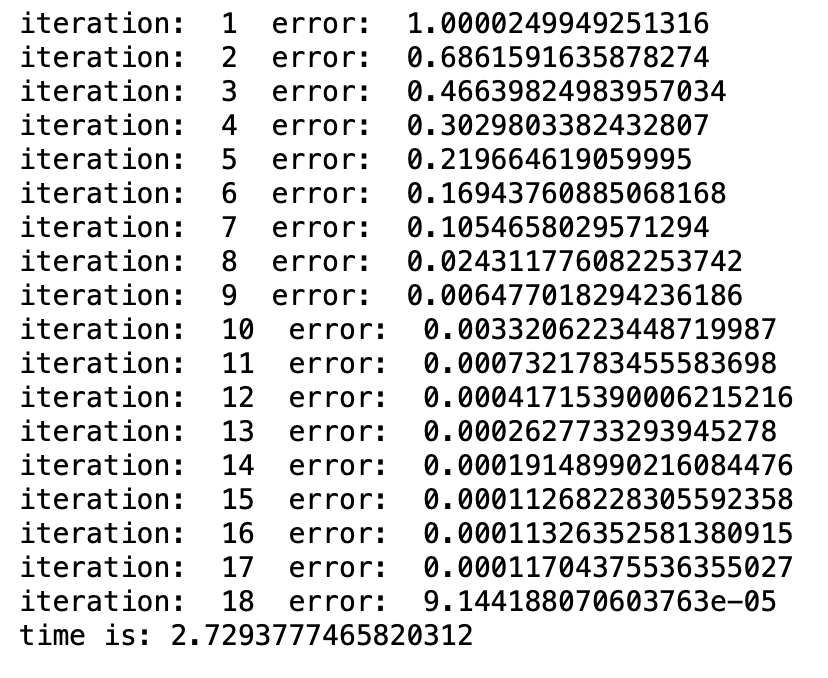
\includegraphics[width=.35\textheight]{qa1.png}
	\caption{Iteration, Termination signal $r^{(k)}$, Running time Report (naive implementation)}
	\label{fig:qa1}
\end{figure}
\\
Moreover, we report the difference between our solution and ground truth in Figure \ref{fig:qa2}.
\begin{figure}[h]
	\centering
	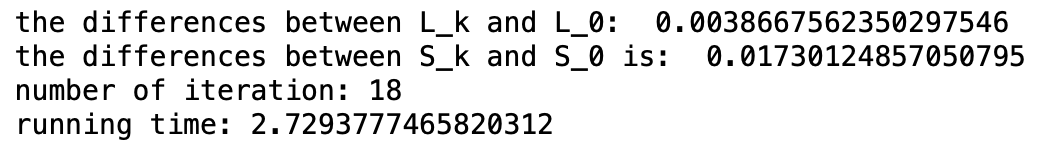
\includegraphics[width=.35\textheight]{qa2.png}
	\caption{Difference between our solution and ground truth Report (naive implementation)}
	\label{fig:qa2}
\end{figure}
\\
\subsection{Q(b): Speed up ADMM via some tricks}
Here, we actually make three different experiments on different choices of $\rho$. Before showing the experiment results, we state of conclusion first. We should choose $\rho$ as an intermediate value. If $\rho$ is too big, then our achieved solution will be very poor although the ADMM algorithm converges very fast. If $\rho$ is too small (close to 1), then our ADMM algorithm will converge very slowly, although our achieved solution can converges to the ground truth as we want.
\subsubsection{$\rho=3$, which is an intermediate value (our interested scenario)}
Here, we choose $\rho=3$ to conduct experiments.
\begin{figure}[h]
	\centering
	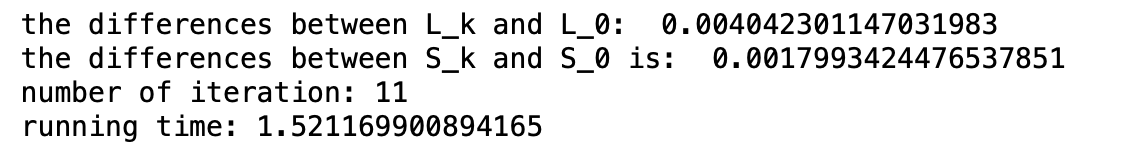
\includegraphics[width=.47\textheight]{qb1.png}
	\caption{Error, Iteration, Running time Report ($\rho=3$)}
	\label{fig:qb1}
\end{figure}
\\
As shown in Figure \ref{fig:qb1}, with good choice of $\rho$, the ADMM algorithm is able to converge faster. We only need 11 iteration in this speed-up version, while 18 iteration is required for naive implementation. Moreover, from the difference reported, we can verify that, the achieved solution correctly converges to the ground truth.
\subsubsection{$\rho=4$, which is too big (bad case)}
Here, we choose $\rho=4$ to conduct experiments.
\begin{figure}[h]
	\centering
	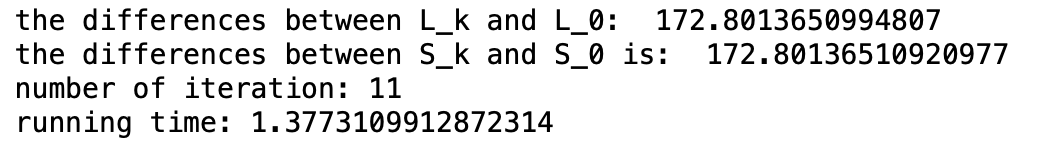
\includegraphics[width=.47\textheight]{qb2.png}
	\caption{Error, Iteration, Running time Report ($\rho=4$)}
	\label{fig:qb2}
\end{figure}
\\
As shown in Figure \ref{fig:qb2}, when we set $\rho$ too big, our ADMM algorithm \textbf{will not converge to the ground truth} from the reported difference. Moreover, it can be also observed that, the ADMM algorithm converges very fast, which only requires 11 iteration for convergence.
\subsubsection{$\rho=1.1$, which is too small (bad case)}
Here, we choose $\rho=1.1$ to conduct experiments.
\begin{figure}[h]
	\centering
	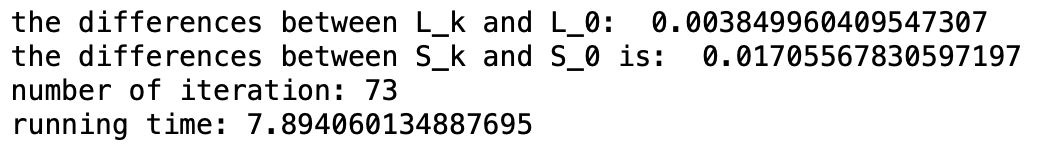
\includegraphics[width=.47\textheight]{qb3.png}
	\caption{Error, Iteration, Running time Report ($\rho=1.1$)}
	\label{fig:qb3}
\end{figure}
\\
As shown in Figure \ref{fig:qb3}, when we set $\rho$ too small, our ADMM converges \textbf{even more slowly compared with the naive implementation}. The reason is, our initialization for $\sigma$ is the inverse of largest eigenvalue, which is a very small value in general. If the increasing rate $\rho$ is also small, e.g., $\rho=1.1$, then $\sigma$ will keep small for a long time, which will restrict the convergence of our algorithm. However, our achieved solution can correctly converge to the ground truth.
\subsection{Q(c): Application of foreground-background segmentation}
Based on the previous discussion, here we set $\rho=3$ to achieve the trade-off between convergence speed and solution quality.
\begin{figure}[!h]
	\centering
	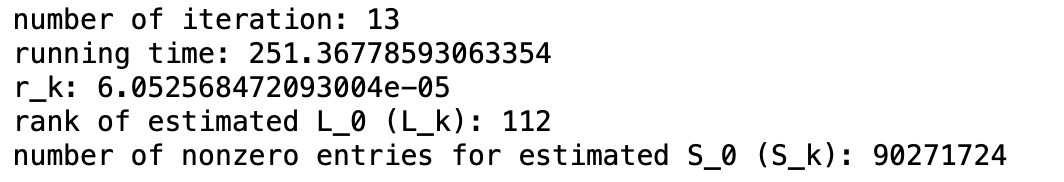
\includegraphics[width=.47\textheight]{qc1.png}
	\caption{Iteration, Running time, Error, Rank and Number of non-zero entries Report ($\rho=3$)}
	\label{fig:qc1}
\end{figure}
\\
Moreover, we report our whole learning trajactory in Figure \ref{fig:qc2}:
\begin{figure}[!h]
	\centering
	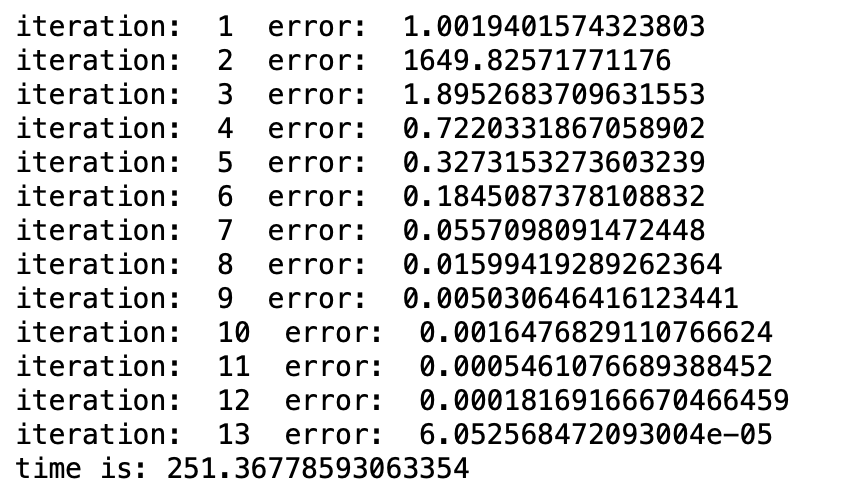
\includegraphics[width=.35\textheight]{qc2.png}
	\caption{Whole Learning Trajactory ($\rho=3$)}
	\label{fig:qc2}
\end{figure}
\subsection{Q(d): Visualize M[:, 19], L[:,19], S[:,19]}
Firstly, we show the total pictures M[:,19], which is the 20-th frame in the video in Figure \ref{fig:qd1}.
\begin{figure}[!h]
	\centering
	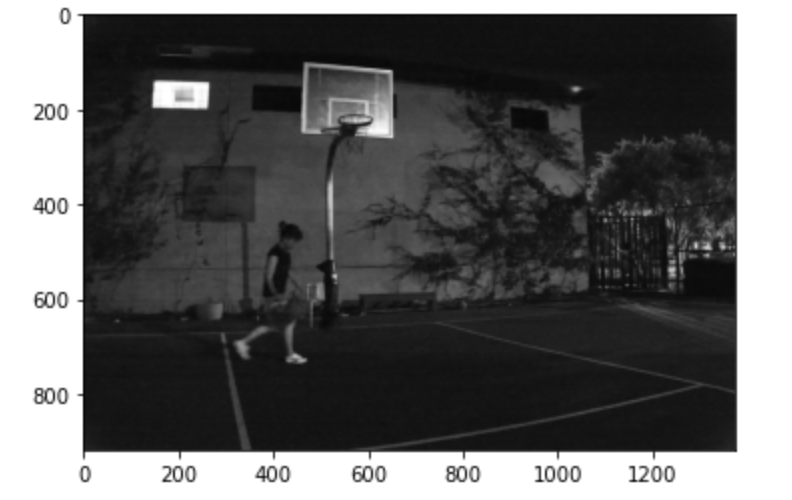
\includegraphics[width=.35\textheight]{qd1.png}
	\caption{20-th frame in the video, M[:,19]}
	\label{fig:qd1}
\end{figure}
\\
Secondly, we show our separation result for the background and person.
\begin{figure}[!htbp]
	\centering
	\subfigure[20-th background frame]{
		\label{fig:subfig:mpfh1} %% label for first subfigure
		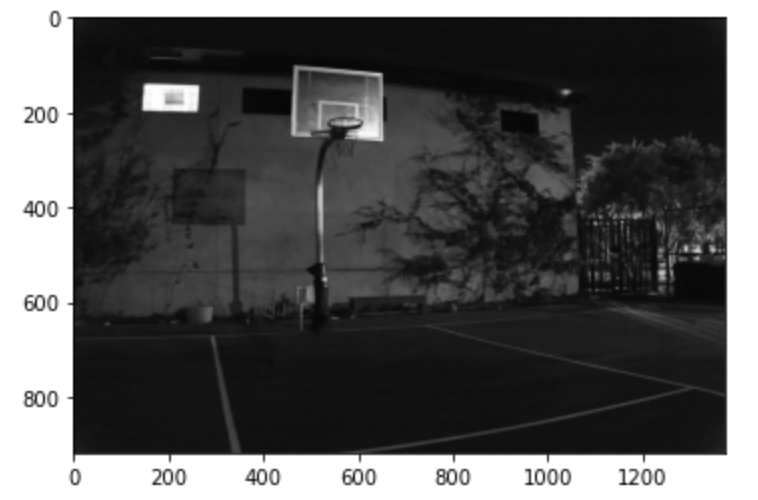
\includegraphics[width=3in]{pd2.png}}
	\subfigure[20-th person frame]{
		\label{fig:subfig:mpfh2} %% label for second subfigure
		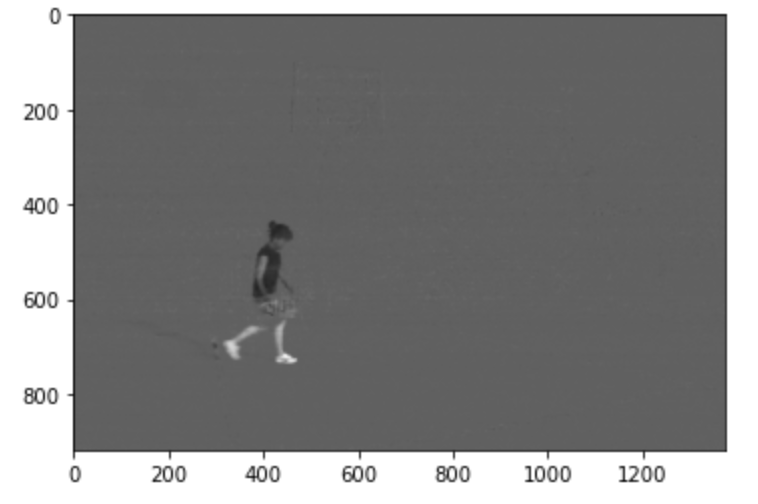
\includegraphics[width=3in]{qd3.png}}
	\caption{20-th Background and Person Frame, L[:,19] and S[:,19]}
	\label{MPFH_hyperparameter} %% label for entire figure
\end{figure}
\subsection{Q(e): Making a Background Video and Moving Object Video}
For this part, we will attach our 'background.avi' and 'people.avi' file. We successfully apply 'cv2' to visualize the result as videos.
\end{document}